\documentclass[]{book}
\usepackage{lmodern}
\usepackage{amssymb,amsmath}
\usepackage{ifxetex,ifluatex}
\usepackage{fixltx2e} % provides \textsubscript
\ifnum 0\ifxetex 1\fi\ifluatex 1\fi=0 % if pdftex
  \usepackage[T1]{fontenc}
  \usepackage[utf8]{inputenc}
\else % if luatex or xelatex
  \ifxetex
    \usepackage{mathspec}
  \else
    \usepackage{fontspec}
  \fi
  \defaultfontfeatures{Ligatures=TeX,Scale=MatchLowercase}
\fi
% use upquote if available, for straight quotes in verbatim environments
\IfFileExists{upquote.sty}{\usepackage{upquote}}{}
% use microtype if available
\IfFileExists{microtype.sty}{%
\usepackage{microtype}
\UseMicrotypeSet[protrusion]{basicmath} % disable protrusion for tt fonts
}{}
\usepackage[margin=1in]{geometry}
\usepackage{hyperref}
\hypersetup{unicode=true,
            pdftitle={Lecture Notes for Biology of Wildlife Populations},
            pdfauthor={Andrew Tyre},
            pdfborder={0 0 0},
            breaklinks=true}
\urlstyle{same}  % don't use monospace font for urls
\usepackage{natbib}
\bibliographystyle{apalike}
\usepackage{longtable,booktabs}
\usepackage{graphicx,grffile}
\makeatletter
\def\maxwidth{\ifdim\Gin@nat@width>\linewidth\linewidth\else\Gin@nat@width\fi}
\def\maxheight{\ifdim\Gin@nat@height>\textheight\textheight\else\Gin@nat@height\fi}
\makeatother
% Scale images if necessary, so that they will not overflow the page
% margins by default, and it is still possible to overwrite the defaults
% using explicit options in \includegraphics[width, height, ...]{}
\setkeys{Gin}{width=\maxwidth,height=\maxheight,keepaspectratio}
\IfFileExists{parskip.sty}{%
\usepackage{parskip}
}{% else
\setlength{\parindent}{0pt}
\setlength{\parskip}{6pt plus 2pt minus 1pt}
}
\setlength{\emergencystretch}{3em}  % prevent overfull lines
\providecommand{\tightlist}{%
  \setlength{\itemsep}{0pt}\setlength{\parskip}{0pt}}
\setcounter{secnumdepth}{5}
% Redefines (sub)paragraphs to behave more like sections
\ifx\paragraph\undefined\else
\let\oldparagraph\paragraph
\renewcommand{\paragraph}[1]{\oldparagraph{#1}\mbox{}}
\fi
\ifx\subparagraph\undefined\else
\let\oldsubparagraph\subparagraph
\renewcommand{\subparagraph}[1]{\oldsubparagraph{#1}\mbox{}}
\fi

%%% Use protect on footnotes to avoid problems with footnotes in titles
\let\rmarkdownfootnote\footnote%
\def\footnote{\protect\rmarkdownfootnote}

%%% Change title format to be more compact
\usepackage{titling}

% Create subtitle command for use in maketitle
\newcommand{\subtitle}[1]{
  \posttitle{
    \begin{center}\large#1\end{center}
    }
}

\setlength{\droptitle}{-2em}
  \title{Lecture Notes for Biology of Wildlife Populations}
  \pretitle{\vspace{\droptitle}\centering\huge}
  \posttitle{\par}
  \author{Andrew Tyre}
  \preauthor{\centering\large\emph}
  \postauthor{\par}
  \predate{\centering\large\emph}
  \postdate{\par}
  \date{2016-12-26}

\usepackage{booktabs}

\begin{document}
\maketitle

{
\setcounter{tocdepth}{1}
\tableofcontents
}
\chapter{Prerequisites}\label{prerequisites}

I assume you have installed R and RStudio to run examples shown in each
chapter.

I originally set out to write this book because no existing population
dynamics texts had the right mix of topics, or didn't address management
related questions, or were far too advanced for an undergraduate
audience.

My educational objectives for the course, and for the curriculum in
which it is embedded, are as follows.

\begin{enumerate}
  \item Estimate the abundance of a species witin a specific geographical area, and critically evaluate the utility of abundance estimates.
  \item Evaluate the impacts of habitat change on future population abundance. 
  \item Assess how changes in harvest regulations will affect population abundance.
  \item Assess the effect of competitors, predators and other species on a focal species.
  \item Predict the consequences of alternative management actions in a Structured Decision Making framework using simple population models.
  \item Identify the management decision(s) and the decision maker(s) relevant to a wildlife issue. 
  \item Articulate the objectives of stakeholders along a means/ends continuum.
  \item Enumerate available management actions and assemble alternative strategies.
  \item Make tradeoffs between competing objectives to select a preferred management strategy in an SDM framework.
\end{enumerate}

I think objectives 2, 3 and 4 could be subsumed into objective 5, but
I've left them broken out for the moment. Objectives 6, 7, 8 and 9
relate directly to using the PrOACT model of Structured Decision Making.
Objective 7 is the same as Larkin's proximate/ultimate distinction, I
think. NRES 311 currently addresses completely or at least introduces
1-3 and 6-9; I'm not sure about 4.

\chapter{The fundamental law of population
dynamics}\label{chap:fundamental}

\begin{equation}
  \Delta N = B - D + I - E
  \label{eq:fundamental}
\end{equation}

This simple equation governs all changes in single species populations.
The change in the abundance of a population in a given area across an
interval of time \(\Delta\), \(\Delta N\), is the sum of the number of
births \(B\), the number of deaths \(D\), the number of immigrants, or
individuals arriving in the area from outside, \(I\), and the number of
emigrants, individuals leaving the area, \(E\). As the interval of time
gets smaller, we can write the fundamental law as a rate

\begin{equation}
N' = bN - dN + i - e
\label{eq:fundamental2}
\end{equation}

where we've replaced the number of births and deaths with the products
of the population abundance, N, and a per capita rate of birth and
death. We've left immigration and emigration as fixed rates. The
apostrophe notation for N means ``instantaneous rate of change'', that
is, the rate when the time interval \(\Delta \rightarrow 0\).

Where things get interesting is when one or more of the rate constants
in (\eqref{eq:fundamental2}) or amounts in (\eqref{eq:fundamental}) on the
right hand side of these equations are not constant. In particular, when
they depend on \(N\), or on the abundance of other species, the dynamics
of populations get very interesting.

\section{The laws of nature}\label{the-laws-of-nature}

The title of this chapter describes equation (\eqref{eq:fundamental}) as a
``law'' -- what do I mean by law? Is it something that was out there,
waiting to be discovered by humans, independent of our existence and
thought? Or was it created by our thinking of it, consistent with
reality but not of reality? Joe Rosen, formerly professor of physics at
Tel Aviv University and the University of Central Arkansas, spent an
entire volume thinking hard about these issues \citep{rosen2010lawless}.
His categorization of reality and what we can know about it is useful
and easy to follow, so I will use it here. He begins with the notion
that there is an objective reality that exists independent of our
existence. The primary reason for this observation is the simple fact
that nature pushes back. Imagine a world where you can fly; wouldn't it
be marvelous! If the world were not objective, but merely a construct of
our imagination (a view of reality known as solipsism), then you could
create this world, and fly. Unfortunately nature pushes back, and you
will fall to the ground. So objective reality constrains what we can do.

The opposite of objective is subjective. Our inner thoughts and feelings
are subjective, that is, they are known only to us as individuals. You
might tell me what you are thinking or feeling, but I have no
independent way of verifying that information. Beliefs about objective
reality are similarly subjective, in that two people can have different
beliefs about reality. However, it is possible for us to conduct
\emph{reality checks} on our beliefs about reality. If enough of us get
together to check our beliefs, and over time, agree to a consensus
belief that passes reality checks, then this is about as close to
objective knowledge as we can get. Rosen calls this form of knowledge
\emph{intersubjective}; it is different from subjective belief by virtue
of its broader consensus amongst many people, and yet not fully
objective by virtue of the fact that it was formed from our subjective
perceptions of reality.

Intersubjective knowledge is socially constructed knowledge, but is not
consistent with the the post-modernist position that all reality is
socially constructed. Our socially constructed, intersubjective beliefs
are constrained by objective reality -- not everything is possible. Even
if a diehard post-modernist could convince a group of a 1000 people that
she could fly unaided, she would not be able to do so.

In the field of wildlife management science, the goal is the production
of ``reliable knowledge'' \citep{romesburg1981wildlife} to use in making
management decisions. It is not uncommon to see exhortations from
leaders in the field to make science based decisions, presumably a call
to use reliable, or intersubjective, knowledge to decide which course of
action should be followed. Unfortunately, as we will see in many
examples throughout this book, people do not make decisions like that.
Our subjective beliefs about many things, from religion to justice,
affect what we think should be done. Inevitably, the more people are
affected by a decision or policy related to wildlife management, the
more political (i.e.~subjective) the decision or policy will become.

So a \emph{law} of population dynamics is well tested intersubjective
knowledge, or reliable knowledge, that we can use to make predictions
about the consequences of management actions. As you will see below, a
law will also have assumptions that must be met in order for it to
apply.

\section{The nature of models of
nature}\label{the-nature-of-models-of-nature}

Almost all of the equations in this book, other than the fundamental
equation, are models of nature. That is, they are deliberate
simplifications of what is really going on out in nature. If our models
were exact replicas of nature, then we would have as much trouble
understanding the model as we have understanding nature! It is easy to
get caught up in the thrill (OK, easy for people who build models) of
adding ever more biological realism to a model. But this does not
necessarily help us make decisions in the face of complexity.

A consequence of this deliberate simplification is that all models are
in fact, fictitious. This might seem surprising. After all, works of
fiction are by definition false. Not true. How can something that is
known to be false help us understand nature? This is a problem that so
vexed early philosophers of science that they deliberately ignored it
for the better part of a century. Fortunately for the science of
population dynamics, this philosophical high-mindedness did not stop
scientists from using models to understand nature. Statistician George
Box put it this way:

\begin{quote}
All models are wrong. Some models are useful. \citep{box1976science}.
\end{quote}

The key is identifying which models are useful. In this book the utility
of a model is measured by the extent to which the model allows us to
forecast the future consequences of management decisions.

\section{Deaths}\label{deaths}

Of all the biological processes in the fundamental equation, the
simplest one to get a handle on is \(D\), the number of deaths in a
period of time. A great deal of fisheries and wildlife management
involves directly manipulating \(D\) through harvest or culling, or
indirectly manipulating \(D\) through habitat management.

Consider the problem of stocking a lake with walleye fingerlings. From
past research at this lake, we know that the instantaneous mortality
rate is \(d = 0.01 week^{-1}\). If a hatchery manager wants to stock
10,000 fingerlings, how many will survive one year? We have three pieces
of information -- the rate of mortality, the initial number of fish, and
the period of time. In continuous time, assuming that there are no
births, emigration or immigration

\begin{equation*}
N' = - dN 
\end{equation*}

This is an equation for the rate of change in a variable where the
variable itself (\(N\)) is multiplied by a constant. This is the
equation for exponential decay. The solution to that equation is

\begin{equation*}
N_t = N_0 e^{-dt}
\label{eq:deaths}
\end{equation*}

We can substitute in the values for our problem, where N0 = 10000 and t
= 52 weeks, which gives us

\begin{equation*}
N_{52} = 10000 e^{-(0.01)(52)} = 5945 fingerlings
\end{equation*}

In nature, the result will almost certainly not be exactly 5945
fingerlings. We do not know \(d\) exactly, \(d\) might not be constant
over the course of the year, and indeed, the process of mortality itself
is not \emph{deterministic}. We cannot know exactly how many fingerlings
will encounter a channel catfish during the year; only that some will
with catastrophic results for the fingerlings! The number 5945 is an
\emph{expected value}, in the sense of Chapter \ref{chap:abundance}.

Instead of an instantaneous mortality rate, we might have a discrete
time rate estimated from a mark-recapture program. In that case we would
have a per capita mortality rate \(d_{\Delta t}=e^{-d \Delta t}\) Note
that the discrete time rate depends on the interval over which it is
estimated.

\section{Births}\label{births}

The second term in the fundamental equation that we must have is the
number of births in a single unit of time, \(B\). There is little that
can be done to manage \(B\) directly; most wildlife management efforts
can at best manipulate \(B\) indirectly by altering the habitat. There
are instances where preventing births through contraception is a useful
management strategy for over abundant species, but it is often more
expensive than manipulating \(D\).

In the continuous time form, the rate of change in N from births is

\begin{equation*}
N' = bN 
\end{equation*}

where b is the per capita rate of births per unit time. The population
size after some interval of time \(t\), \(N_t\) will be given by

\begin{equation}
N_t = N_0 e^{bt}
\label{eq:births}
\end{equation}

There are not very many species where births occur continuously (put in
a box describing one of each type). Equation (\eqref{eq:births}) is an
approximation of what usually occurs with wildlife species, especially
wildlife in temperate and polar systems. There are many circumstances in
which this approximation is acceptable, but we must never forget that it
is an approximation, not the objective reality. In Chapter
\ref{chap:structured} we will examine alternative approximations to the
birth process that more closely match the biological reality.

\section{Turchin's law of population
inertia}\label{turchins-law-of-population-inertia}

With births and deaths, we can proceed to construct the simplest
possible model of population dynamics. In order to do so we must make an
assumption about the remaining two pieces of the fundamental equation,
\(I\) and \(E\), the number of individuals moving into and out of the
population. We have a couple of choices here, but let us start with the
simplest assumption: \(I = E = 0\). That is, we will assume that no
individuals move into or out of the population. The population is
\emph{closed} to emigration and immigration. With this assumption, the
fundamental equation in continuous time reduces to

\begin{equation}
N' = bN - dN =(b-d)N = rN
\label{eq:definer}
\end{equation}

where we've defined a new constant \(r\), the difference between the per
capita birth and death rates. This constant \(r\) is so important in
population dynamics that it has a special name -- the \emph{intrinsic
rate of population growth}. Notice that equation (\eqref{eq:definer})
looks a lot like equation (eq:deaths) and (eq:births). It is the
equation for exponential growth or decay, and we know the solution for
that:

\begin{equation}
N_t = N_0 e^{rt}
\label{eq:expgrowth}
\end{equation}

This is the equation for exponential population growth, and it is the
simplest possible population model. When \(r > 0\), the population will
increase, and when \(r < 0\) the population will decrease (Figure 1).
Looking back at eq. \eqref{eq:definer}, we can see that \(r > 0\) when the
per capita birth rate is greater than the per capita death rate. That
makes sense -- in order for the population to increase the number of
births must exceed the number of deaths. Conversely, \(r < 0\) when the
per capita birth rate is less than the per capita death rate. The most
important thing to recognize here is that the difference between a
population growing or decaying is determined by the relative magnitudes
of b and d. Measuring either one alone does not tell us whether the
population will increase or decrease. What happens if \(r\) is exactly
equal to zero? The population will neither increase nor decrease, but
remain at exactly the same level.

Turchin's law of population inertia states: in the absence of other
forces, a population will continue to grow (or decline) exponentially
\citep{turchin2003complex}. Equation (\eqref{eq:expgrowth}) tells us the
rate at which the population will grow or decline. The important part of
the law is the first phrase, ``in the absence of other forces''.

That is, assuming that the per capita birth and death rates remain
constant, unaffected by other processes, then the law of population
inertia holds. Much of the remainder of this book focuses on determining
when the law of population inertia does not hold.

\begin{figure}[htbp]
\centering
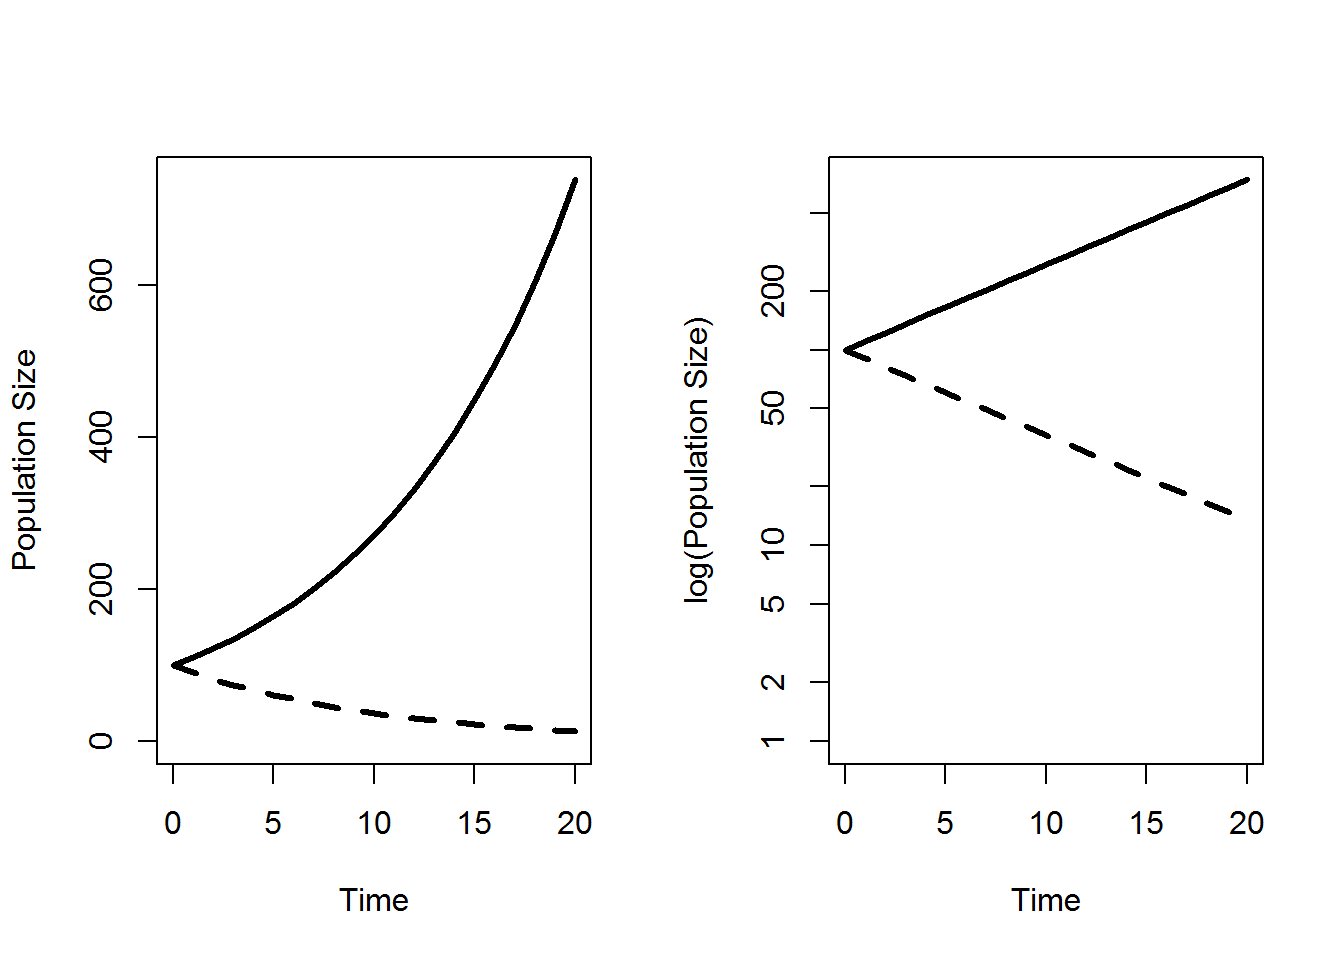
\includegraphics{NRES450-LectureNotes_files/figure-latex/expgrowth-1.pdf}
\caption{\label{fig:expgrowth}Population growth over time r is greater than
or less than zero. The right hand panel shows the same curves on a log
scale.}
\end{figure}

There is one additional property of the exponential model of population
dynamics that makes it useful as a touchstone for analyzing changes in
numbers. If we take the logarithm of both sides of Equation
(\eqref{eq:expgrowth}), we obtain

\begin{equation*}
ln(N_t) = ln(N_0) + rt
\end{equation*}

which has the same form as the equation of a straight line. The
y-intercept of the graph is the logarithm of the population size when
\(t=0\). Plotting the logarithm of \(N_t\) against time will then have a
straight line with a slope of \(r\). This is a very easy way to check if
a particular time series is well approximated by the exponential
population model.

\section{\texorpdfstring{Estimating
\(r\)}{Estimating r}}\label{estimating-r}

If this constant \(r\) is so important, how do we figure out what value
to use? Later we will build up an estimate of \(r\) from detailed life
history information. It can also be done in a ``back of the envelope''
way as long as we have two estimates of population size at different
times. We start with equation (\eqref{eq:expgrowth}), and rearrange it to
solve for \(r\)

\begin{equation}
\begin{split}
\frac{N_t}{N_0} & = e^{rt} \\
ln\left(\frac{N_t}{N_0}\right)  & = rt \\
r & = ln\left(\frac{N_t}{N_0}\right) /  t 
\end{split}
\end{equation}

So our first estimate of \(r\) is the log of the ratio of population
estimates, divided by the number of time periods between the two
estimates. This estimate assumes that the law of population inertia held
during the intervening \(t\) time periods. As an example, let us carry
out these calculations for the herd of Muskox (\emph{Ovibus moschatus})
on Nunivak Island, Alaska. Muskox were extirpated from the Arctic slope
of Alaska in the late 19\textsuperscript{th} century, and efforts to
reintroduce them from populations in Greenland began in the 1930's. In
1947 David Spencer of the Bureau of Sport Fisheries and Wildlife in
Alaska began an annual survey of the Nunivak Island population
\citep{spencer1970muskox}. He recorded a total of 49 animals in 1947,
and in 1965 he counted 514 animals total. Assuming that the law of
population inertia held during those 18 years, we find

\begin{equation}
r = ln\left(\frac{N_t}{N_0}\right) /  t = 
    ln\left(\frac{514}{49}\right)  / 18 = 
    \frac{ln(10.49)}{18} = 0.13 \, years^{-1}
\end{equation}

How should we interpret that estimate? The change in a population over 1
year is \(Ne^r\), so the factor \(e^r\) is the percentage change in
population size. In this case, \(e^r = 1.138\), or about a 14 \% change
per year. A useful approximation to remember is that when \(r\) is close
to 1, then \(e^{r} \approx 1+r\), so you can think of \(r\) as a
percentage change in population size per year as long as it isn't too
large. In the musk-ox case the error in this approximation is 1
percentage point.

With this estimate of \(r\) in hand, there are several things we can do.
For example, what if we want to predict the number of animals on the
island after another 3 years, assuming population growth holds at the
same rate?

\begin{equation}
N_3 = 514 e^{(0.13)(3)} = 514(1.48) = 759\,muskox
\end{equation}

This is quite useful as a benchmark for management. If we go back in 3
years and there are a lot fewer, or a lot more muskox than we expected,
then we would have to conclude that ``all other forces'' were not in
fact zero, and that would start us on a useful search for what might
have changed. In fact, in 1968 there were 714 animals. Is that a lot
fewer than expected? In order to answer that question, we need to
address an important issue -- indeterminism -- which we will begin in
the next chapter.

Another easy calculation to do is finding the \emph{doubling time} for a
population. This is the number of years for the population to double in
size. The key here is to recognize that a population has doubled when
\(N_t = 2N_0\). We substitute \(2N_0\) into eq. \eqref{eq:expgrowth} and
solve for \(t\)

\begin{equation}
\begin{split}
\frac{2N_0}{N_0} & = e^{rt} \\
ln\left(2\right)  & = rt \\
t & = \frac{ln\left(2\right)}{r}\,.
\end{split}
\label{eq:double}
\end{equation}

For the musk ox we get \(t = ln(2)/0.13 = 5.3 \, years\) for the
population to double in size. This calculation is very handy for guiding
management expectations. If we desire a population to be 10\% larger, we
can calculate how many years that will take by replacing the constant 2
in eq. \eqref{eq:double} with 1.1.

\section{Glossary}\label{glossary}

\begin{enumerate}
  \item **Deterministic processes** have only a single outcome given complete knowledge of the state of the system.
  \item **Expected value** of a random variable is the mean value, or the 1st moment of the distribution.
  \item **Instantaneous mortality rate** the rate at which mortality events occur when the interval of time is allowed to shrink towards zero.
  \item **Solipsism** A metaphysical viewpoint that asserts reality is only the result of our imaginations.
\end{enumerate}

\section{Exercises}\label{exercises}

\begin{enumerate}
  \item An index of the Bald Eagle population in Illinois [@havera1988distribution] grew from 188 individuals in 1970 to 569 individuals in 1987. Assuming a closed population with constant birth and death rates through this period, what was the annual population growth rate?
  \item For the same population of Bald Eagles in Illinois, how many eagles would you expect in 1984?
  \item If the actual population count in 1984 was 930, what could you conclude about this population?
  \item In how many years would you expect the Bald Eagle population to double in size after 1987?
  \item Wildlife managers at an east coast wildlife refuge want their population of Piping Plovers to increase by 20\% in 5 years. Their estimated value of $r = 0.01$ without changing any management strategies. Can they achieve their objective? What value of $r$ would allow them to achieve their objective?
\end{enumerate}

\bibliography{packages,book}


\end{document}
